\chapter{Framework di Anonimizzazione}

\nt{Molti di questi Framework sono superati, ai giorni nostri \fancyglitter{differential privacy} ha soppiantato tutti gli altri.}

\section{Il Problema dell'Anonimità}

\paragraph{Problema:}

\begin{itemize}
  \item Molte agenzie, istituzioni, organizzazioni, etc. rendono pubblicamente disponibili dati sensibili riguardanti persone: 
    \begin{itemize}
      \item Molti microdata per le analisi. 
      \item Spesso la legge richiede la loro anonimizzazione.
    \end{itemize}
  \item I microdata vengono \fancyglitter{sanificati}. 
  \item Non è sufficiente per preservare la privacy:
    \begin{itemize}
      \item Suscettibili a \fancyglitter{linking attack}. 
      \item Databases pubblici possono rilevare identità "segrete".
    \end{itemize}
\end{itemize}

\subsection{Linking Attack}

Nel 2001, Latanya Sweeney riuscì a reidentificare i record medico del governatore del Massachussetts: 
\begin{itemize}
  \item Il Massachussetts colleziona e pubblica dati medici sanificati per gli impiegati statali. 
  \item I dati dei votanti registrati sono pubblicamente disponibili.
\end{itemize}

\begin{figure}[h]
    \centering
    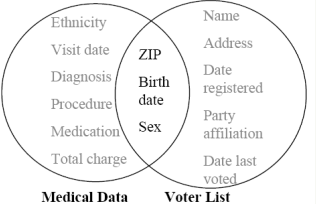
\includegraphics[scale=0.41]{03P/LA.png}
    \caption{Linking Attack del 2001.}
\end{figure}



\section{K-Anonimity}
